\section{Literature} \label{sec:Literature}
% In the next section, present a summary of what other authors have written on your topic.

The latest ``Consumer Credit Card Market'' report from the \citet{cfpb:2023} contains a wealth of information about how Americans use their credit cards, separated by FICO credit scores according to the levels shown in Table~\ref{tab:FICO}.
The CFPB reports that more than 90 percent of the purchase volume is on rewards cards, and that the average rewards-earning account contained \$156 in 2022. 
But, as we can see in Fig.~\ref{fig:CFPBRewardsBalances}, accounts with high credit scores have considerably higher rewards balances compared to accounts with low credit scores. 
The CFPB also finds that people with prime plus or superprime credit scores keep zero, or very low, revolving balances, while their purchase volumes and payment rates are actually the highest. 
This is consistent with practicing good financial habits in order to enjoy the benefits of credit card rewards and reach a high FICO score.%
\footnote{Although the exact algorithm is proprietary, there are many online resources that explain what a FICO score consists of, and how one can improve it, e.g. \url{https://www.myfico.com/credit-education/credit-scores}.}
The most important habit regarding rewards is to pay off statement balances \emph{in full} by the due date each month (so no interest on revolving balances is paid). This implies only using credit cards for purchases that you can afford to pay off completely the next month.

% Table of FICO thresholds according to the CFPB and Agarwal et al. (2023)    
\begin{table}[t!]
    \centering
    \begin{tabular}{ r c c } 
        \hline
        & CFPB & Agarwal \emph{et al.} (2023) \\ 
        \hline
        deep sub-prime & $<580$ & \\
        sub-prime & 580--619 & $<660$ \\ 
        near-prime & 620--659  & 660--719 \\ 
        prime & 660--719 & 720--779 \\ 
        prime plus & 720--799 & \\
        super-prime & $>799$ & $>779$ \\ 
        \hline
    \end{tabular}
    \caption{FICO score thresholds used by the CFPB and \citet{agaretal:2023}.}
    \label{tab:FICO}
\end{table}


\begin{figure}[t!h]
    \begin{center}
    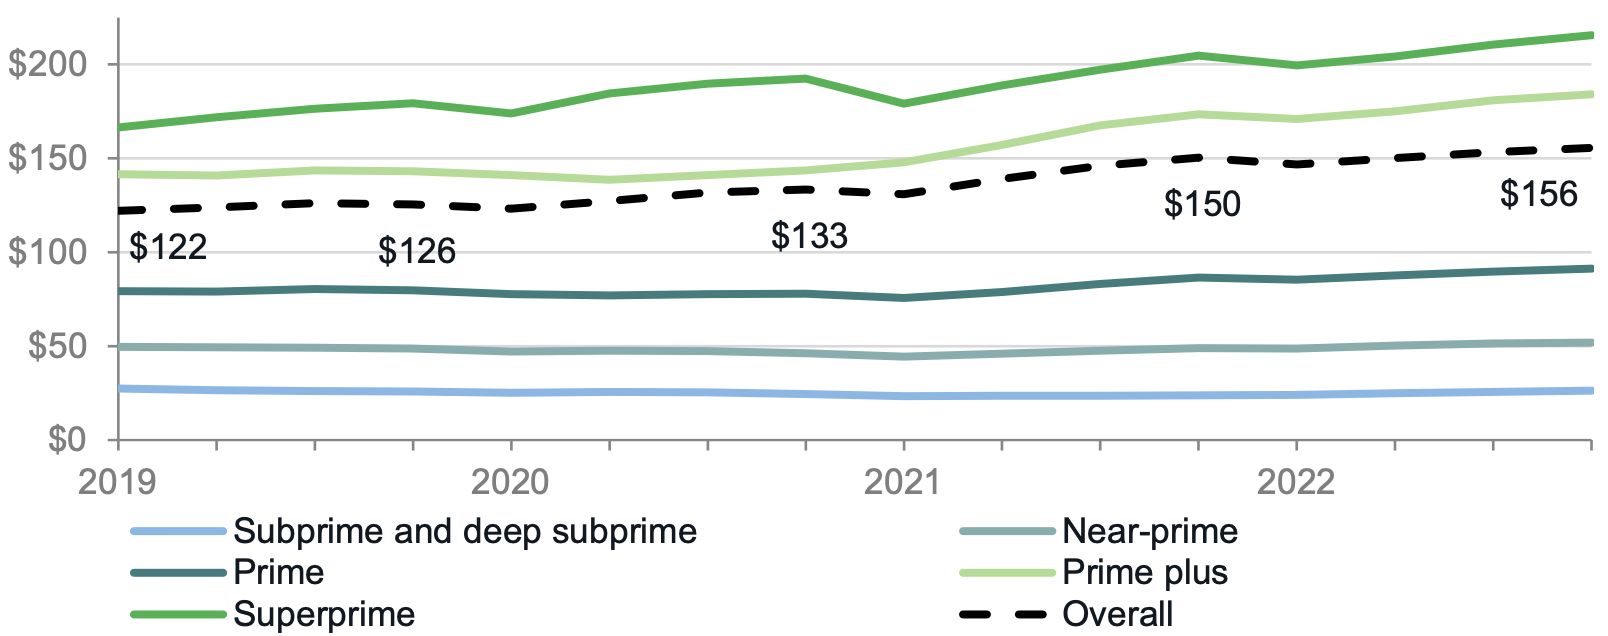
\includegraphics[width=0.8\textwidth]{../Misc/CFPBFig2_DollarPerAccount.png}
    \caption{Quarterly dollar value of average rewards balances for different credit scores. Source:~\citet{cfpb:2023}.}
    \label{fig:CFPBRewardsBalances}
    \end{center}
\end{figure}

While it is true that applying for new credit cards results in the banks ``pulling'' the applicant's credit report, lowering the credit score, it is important to note that this effect is only temporary. In the long run, opening many credit cards to optimize rewards can actually have a positive impact on credit scores, as the ``utilization ratio'' per card is lowered (the amount of spending on the card as a percentage of the credit limit). 
As an example, Fig.~\ref{fig:FICOTimeline} shows a time series of my personal credit scores with the dates of nine credit card applications marked. Even with this above-average number of credit card applications, the overall trend in credit scores is positive.

\begin{figure}[t!h]
    \begin{center}
    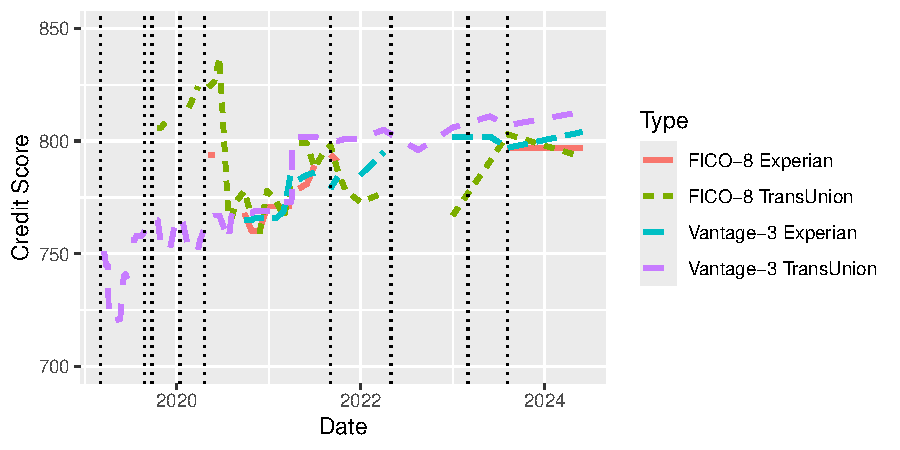
\includegraphics[width=1.0\textwidth]{CreditScoresTimeSeries.pdf}
    \caption{Time series of my personal credit scores. The vertical dotted lines mark the dates when new credit card accounts were opened.}
    \label{fig:FICOTimeline}
    \end{center}
\end{figure}

Regarding the payment structure of rewards programs, Fumiko Hayashi \citeyearpar{hayashi:2009} shows a good overview of the payment fee flows between the merchant, the merchant acquirer (the bank that processes card payments for the merchant), the card issuer (the cardholder's bank) and the cardholder.
In an example where the cardholder makes a \$100 purchase, the merchant receives \$97.50. The \$2.50 in fees is split between the merchant acquirer (\$0.50) and an interchange fee of \$2.00 that is paid from the merchant acquirer to the card issuer. The card issuer pays a fraction of the interchange fee (say \$1.00) as a reward to the cardholder, and also pays the card network (such as Visa or MasterCard), who set the interchange fees.%
\footnote{American Express transactions work differently, as American Express operates its own network and simultaneously acts as both card issuer and merchant acquirer.}
The merchant is likely to pass on these fees as higher retail prices to the consumer (regardless of the payment method). \citet{hayashi:2009} concludes that it is not completely clear who ultimately pays for the rewards programs, but it seems likely that credit card rewards programs are not efficient markets. 
For rewards programs to be Pareto efficient, the use of credit cards would have to lead to cost savings for the merchants (due to less handling of cash, which comes with security risks and depositing costs). 
Only the savings beyond the operating costs of handling credit card transactions would then be returned to customers in the form of rewards, in which case everyone is better off without anyone being worse off. Such a scenario seems unlikely when many merchants complain about interchange fees being too high. 

\begin{figure}[t!h]
    \begin{center}
    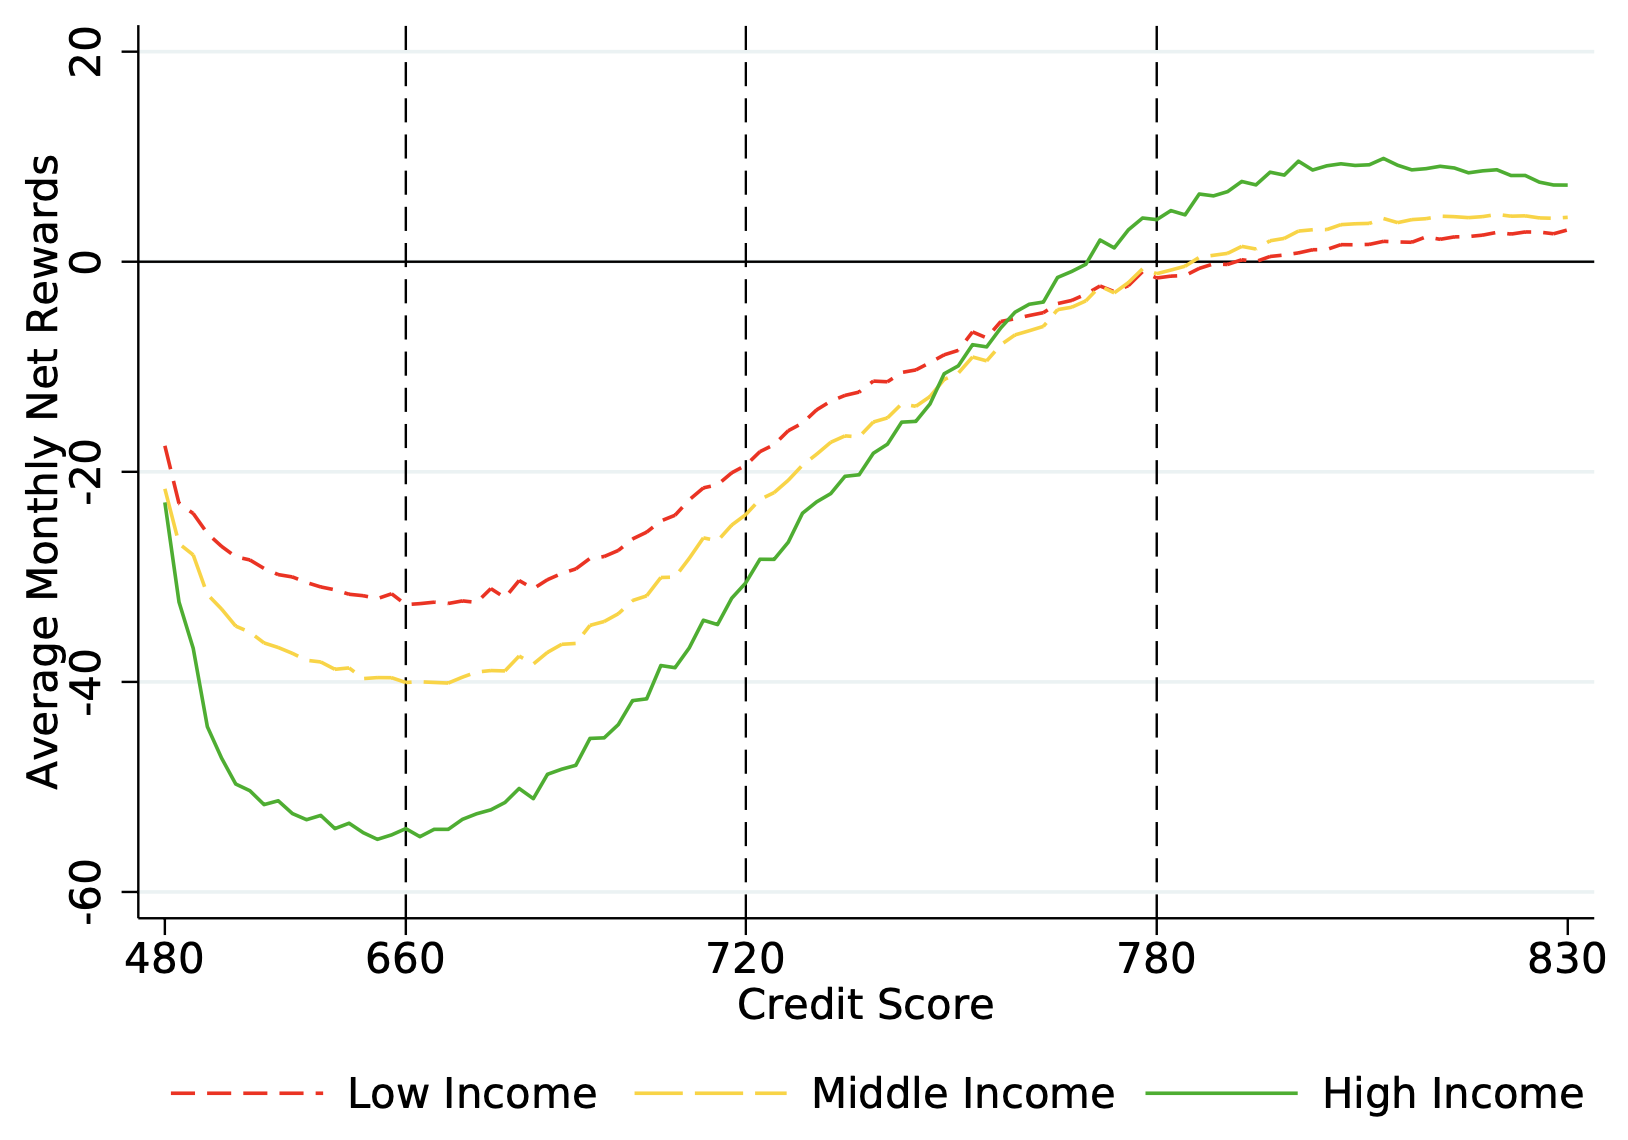
\includegraphics[width=0.7\textwidth]{../Misc/Agarwal_NetRewardsByIncome.png}
    \caption{Average monthly net rewards by income and credit score. Source: \citet{agaretal:2023}.}
    \label{fig:AgarwalRewards}
    \end{center}
\end{figure}

\citet*{schuetal:2010} find that it is cash-using households who are paying for the rewards of card-using households, which, due to the positive correlation between income and use of credit cards, translates to lower incomes paying for the rewards of higher incomes (the ``reverse Robin Hood'' mechanism). 
However, \citet*{agaretal:2023} show that this redistribution takes place from low to high FICO scores \emph{regardless} of income.
As Fig.~\ref{fig:AgarwalRewards} shows, it is primarily the super prime cardholders who have positive monthly net rewards, while the sub-prime and near-prime cardholders pay the most for using rewards cards. Interestingly, high-income, super-prime cardholders benefit the most (\$20.1 in net rewards per month), primarily at the expense of \emph{high-income} cardholders with low credit scores.

\citet*{agaretal:2023} use FICO scores as a proxy for financial sophistication, and conclude that ``sophisticated individuals profit from reward credit cards at the expense of na\"{i}ve customers.''
They also estimate the aggregate annual redistribution to be \$15 billion and find that this redistribution takes place from less to more educated, poorer to richer, and high to low minority areas, widening existing disparities.

% Even though in this project I do not have access to detailed data on people's income, zip codes, and credit card usage, it will be interesting to compare some of these results to a modeling exercise that accounts for different types of credit card users. 

% https://fredblog.stlouisfed.org/2023/10/credit-card-holders-and-their-credit-scores/ 
